\chapter{カラー表現、ハドロン、閉じ込め}

\paragraph{短い序奏。}
群論に戻る前に、恥ずかしながら一つ宣伝をさせていただく。\emph{ブラックホール戦争}は、ブラックホールが量子情報を破壊するかどうかをめぐるスティーブン・ホーキングとの長い論争の物語である。そこにはまた、理論物理学者に特有の残酷さも記録されている。シュレーディンガーの猫だけでなく、サスキンドの魚とその不運なトイレへの旅もそうである。その義務を果たしたので、アリスとボブに戻ろう。アリスはまだ苦しんでいる。ボブがまだ彼女に群論を学ばせているからである。

\lectureoverview{対称性は状態への作用を通じて物理的になる。まず回転から始めて表現と生成子を導入し、次に同じ構成をカラー\(SU(3)\)について繰り返す。カラー表現は結合してハドロンになり、その力学が孤立したカラーが決して観測されない理由を説明する。}

\section{群とそれが作用するもの}

すべての対称性の議論には二つの考え方がある。第一に抽象群がある。すなわち、乗法則、単位元、逆元を備えた操作の集まりである。第二に、それらの操作が作用する対象がある。この二つの考え方は区別できるが、物理学では切り離せない。対称性が重要であるのは、それが物理的状態、場、座標、または観測量を変換するからである。

\begin{classroomqa}
\audiencequestion{群は、抽象的な乗積表としても、物理的対象に作用する行列としても記述されてきた。この二つの部分は切り離せるのだろうか。
\lecturetimestamp{00:01:58}}
\lecturerresponse{それらは記述の異なる水準であるが、完全に関連している。回転は、何を回転させるかを指定する前に、抽象的な操作として存在する。そして物理学は、その同じ操作が特定の系に関連する状態や量にどのように作用するかを問う。行列は、抽象的な乗法則を保ちながら、その具体的な作用を与える。}
\end{classroomqa}

空間回転が最も明快な例を与える。古典的には、同じ回転が粒子の座標に作用しても、磁石の向きに作用しても、その他の任意のベクトルに作用してもよい。量子力学では、状態は線形ベクトル空間に住んでいるので、回転はその空間上の線形演算子によって表現される。\(g\)が抽象群の元を表し、\(D(g)\)がその行列表現を表すならば、整合性とは
\begin{equation}
D(g_1g_2)=D(g_1)D(g_2),
\qquad
D(e)=\boldsymbol 1.
\end{equation}
を意味する。行列は抽象的な操作と同じに見える必要はないが、その乗法は群の乗法を再現しなければならない。
\editorialnote{この準同型の式は、本文で言葉で説明された群の乗法と行列の乗法の対応を明示的に書き表している。}

行列の次元は、抽象群だけによってではなく、状態空間によって決まる。一つの電子のスピンだけを保持するならば、直交する二つの可能性、スピン上向きとスピン下向きがあり、状態は二成分の列ベクトルである。したがって回転は\(2\times2\)行列を通じて作用する。二つのスピン1/2の対象に対しては四つの基底状態があり、
\begin{equation}
\ket{\uparrow\uparrow},\qquad
\ket{\uparrow\downarrow},\qquad
\ket{\downarrow\uparrow},\qquad
\ket{\downarrow\downarrow},
\end{equation}
であり、結合された空間への誘導された作用は四次元である。

おなじみの系列は
\begin{equation}
\begin{array}{c|c|c}
\text{spin} & \text{number of states} & \text{matrix dimension}\\
\hline
0 & 1 & 1\times1\\
\frac12 & 2 & 2\times2\\
1 & 3 & 3\times3\\
\frac32 & 4 & 4\times4
\end{array}
\end{equation}
などである。スピン0の状態は自明な表現をなす。すべての回転がそれをそのままにする。その1行1列の行列は単に\(1\)である。スピン1の状態は三つの成分を持ち、その回転行列はおなじみの三次元ベクトル回転である。より一般に、スピン\(j\)は\(2j+1\)個の状態を持つ。

表現は無限次元にもなりうる。電子のスピンだけでなくその完全な軌道運動を記述するならば、状態はあらゆる位置に対する振幅、あるいは等価に、あらゆる運動量に対する振幅を含む。そのとき回転演算子は波動関数の無限次元空間に作用する。したがって、一つの同じ抽象的回転群が、自明な表現、二次元表現、三次元表現、および無限次元表現を持つ。これが、議論がスピンからカラーへ移るときに再利用する事実である。

\section{なぜスピン回転は特殊ユニタリなのか}

ここで一つの電子スピンに戻り、その軌道運動を捨て去ろう。回転は\(2\times2\)ユニタリ行列\(U\)によって表現され、
\begin{equation}
U^\dagger U=\boldsymbol 1,
\qquad
U^{-1}=U^\dagger.
\label{eq:l4-unitarity}
\end{equation}
である。逆変換は回転を打ち消さなければならず、ユニタリ性はノルム、したがってすべての確率を保存する。

一般の\(2\times2\)複素行列は四つの複素成分、すなわち八つの実パラメータを含む。式~\eqref{eq:l4-unitarity}は四つの独立な実条件を課し、四つのパラメータを残す。通常の空間回転は三つしか持たない。二つのパラメータが軸を選び、一つが角度を選ぶ。したがってユニタリ行列は位相を一つ余分に含む。追加の制限は
\begin{equation}
\det U=1.
\label{eq:l4-det-one}
\end{equation}
である。そのとき数え上げは
\begin{equation}
8-4-1=3.
\end{equation}

行列式が一であるという制限は、乗法の下で安定である。なぜなら
\begin{equation}
\det(AB)=\det A\,\det B.
\end{equation}
二つの行列がそれぞれ行列式が一であるならば、それらの積もまた行列式が一である。この制限はまた、ユニタリ性とも整合する。
式~\eqref{eq:l4-unitarity}の行列式をとると
\begin{equation}
1=\det(U^\dagger U)
=\det(U^\dagger)\det U
=(\det U)^*\det U.
\end{equation}
が得られる。したがって、ユニタリ行列の行列式は単位円上にあり、
\begin{equation}
\det U=e^{i\phi}.
\end{equation}

\begin{classroomqa}
\audiencequestion{ユニタリ性は行列式が実数であることを要求するのだろうか。
\lecturetimestamp{00:12:10}}
\lecturerresponse{いいえ。ユニタリ性が要求するのは、絶対値が1であることだけである。行列式は任意の純粋な位相\(e^{i\phi}\)でありうる。2次元行列の場合、\(U\)に\(e^{-i\phi/2}\)を掛けると、その共通の位相が取り除かれ、行列式1の行列が得られる。}
\end{classroomqa}

実際、もし
\begin{equation}
V=e^{-i\phi/2}U,
\end{equation}
ならば、\(V\)はユニタリのままであり、
\begin{equation}
\det V=e^{-i\phi}\det U=1.
\end{equation}
行列式1のユニタリ行列は\(SU(2)\)をなす。

1つ微妙な点がある。\(SU(2)\)は単に3次元空間における回転の群であると言いたくなるが、対応は2対1である。行列\(U\)と\(-U\)はスピノルに対して異なる作用をするが、通常のベクトルの同じ回転に対応する。したがって
\begin{equation}
SU(2)/\{\boldsymbol 1,-\boldsymbol 1\}\simeq SO(3).
\end{equation}
現在の議論では、局所的な乗法構造と3つの生成子が重要であるが、二重被覆はスピン1/2の回転が2価であることを説明する。

\section{無限小変換とその生成子}

有限回転は、多数の非常に小さな回転から構成することができる。単位元に近い群要素は無限小と呼ばれ、連結な群においては、すべての無限小方向を知ることで、繰り返しの乗法によって有限変換を再構成するのに十分である。物理学にとってさらに重要なのは、これらの無限小変換を生成する演算子が、対称性に対応する保存量であるということである。

単位元に近い要素を
\begin{equation}
U=\boldsymbol 1+i\epsilon T,
\qquad |\epsilon|\ll1.
\label{eq:l4-infinitesimal-u}
\end{equation}
と書く。\(i\)の因子は便利な慣習である。ユニタリ性に代入し、\(\epsilon^2\)の次数の項を捨てると
\begin{align}
(\boldsymbol 1+i\epsilon T)
(\boldsymbol 1-i\epsilon T^\dagger)&=\boldsymbol 1,
\\
i\epsilon(T-T^\dagger)&=0,
\\
T&=T^\dagger.
\label{eq:l4-hermitian-generator}
\end{align}
生成子はエルミートである。量子力学的な観測量がそうでなければならないように。

\begin{figure}[htbp]
\centering
\includegraphics[width=0.62\textwidth]{lecture_04_figure_03.png}
\caption{\(T=T^\dagger\)で終わる、単位元に近いユニタリ性の計算。}
\lectureframe{00:23:28}
\end{figure}

空間回転の場合、3つの独立な無限小軸が存在するため、3つの線形独立な生成子が存在する。任意の方向まわりの小さな回転は、\(x\)、\(y\)、\(z\)まわりの小さな回転から組み立てられる。対応する生成子は角運動量演算子\(J_x,J_y,J_z\)である。それらの交換子は回転の非可換性を符号化しており、
\begin{equation}
[J_i,J_j]=i\epsilon_{ijk}J_k.
\label{eq:l4-angular-momentum-algebra}
\end{equation}
その後、繰り返しの無限小回転によって有限回転が構成される。

我々はユニタリ性を用いたが、まだ行列式1を用いていない。任意の小さな行列\(m\)に対して、
\begin{equation}
\det(\boldsymbol 1+\epsilon m)
=1+\epsilon\,\operatorname{tr}m+O(\epsilon^2).
\label{eq:l4-det-expansion}
\end{equation}

\begin{figure}[htbp]
\centering
\includegraphics[width=0.62\textwidth]{lecture_04_figure_02.png}
\caption{黒板に書き始められたところの、1次の行列式展開。}
\lectureframe{00:21:51}
\end{figure}

式~\eqref{eq:l4-det-expansion}を式~\eqref{eq:l4-infinitesimal-u}に適用すると、
\begin{equation}
\det U
=1+i\epsilon\,\operatorname{tr}T+O(\epsilon^2).
\end{equation}
したがって、特殊ユニタリ条件は
\begin{equation}
\operatorname{tr}T=0.
\label{eq:l4-traceless-generator}
\end{equation}
を要求する。\(SU(2)\)の生成子はまさにトレースがゼロのエルミートな\(2\times2\)行列である。そのベクトル空間の次元は3である。標準的な基底はパウリ行列によって与えられ、
\begin{equation}
\begin{aligned}
\sigma_x&=
\begin{pmatrix}0&1\\1&0\end{pmatrix},
&
\sigma_y&=
\begin{pmatrix}0&-i\\i&0\end{pmatrix},
\\[0.4em]
\sigma_z&=
\begin{pmatrix}1&0\\0&-1\end{pmatrix}.
\end{aligned}
\end{equation}
スピン1/2の表現に対しては\(J_i=\sigma_i/2\)ととることができ、したがって\(\hat{\boldsymbol n}\)まわりの角度\(\theta\)の有限回転は
\begin{equation}
U(\hat{\boldsymbol n},\theta)
=\exp\!\left(-i\theta\,
\hat{\boldsymbol n}\cdot\boldsymbol\sigma/2\right).
\end{equation}
\editorialnote{有限指数関数は、無限小生成子の議論の標準的な完結である。原典はこの式を明示的に書くよりも、繰り返しの小さな回転を強調している。}

\begin{classroomqa}
\audiencequestion{では、トレースがゼロのエルミートな\(2\times2\)行列が3つあるのだろうか。
\lecturetimestamp{00:24:07}}
\lecturerresponse{はい。それらは3つのパウリ行列である。\(3\times3\)特殊ユニタリ行列に対しては、対応する数は8であり、従来の基底は8つのゲルマン行列によって与えられる。}
\end{classroomqa}

\begin{classroomqa}
\audiencequestion{その8は、八道説や8つのグルーオンと同じ``8''なのだろうか。
\lecturetimestamp{00:24:43}}
\lecturerresponse{数学は同じ種類の\(SU(3)\)表現論であるが、どの\(SU(3)\)対称性が作用しているかを特定しなければならない。歴史的な八道説のフレーバー対称性はカラー\(SU(3)\)ではない。8つのグルーオンはカラー\(SU(3)\)の随伴表現に属する。}
\end{classroomqa}

\section{SU(2)からカラーSU(3)へ}

次に、行列を\(2\times2\)から\(3\times3\)へと大きくする。一般の複素\(3\times3\)行列は9個の複素成分をもつので、実パラメータは18個である。条件\(U^\dagger U=\boldsymbol 1\)が9個の実拘束を与え、\(\det U=1\)がさらに1個を除く。したがって
\begin{equation}
18-9-1=8.
\end{equation}
独立な無限小方向は8個あり、トレースがゼロのエルミート生成子も8個ある。\(SU(2)\)とは異なり、この群は通常の3次元空間の回転群ではない。これはカラーに作用する内部対称性である。

これらの表現をクォークに割り当てる前に、複合表現がどのように生じるかを思い出そう。スピン1/2の系を2つ重ね、軌道運動を無視する。積状態は4つあるが、回転は4つすべてを既約に混ぜ合わせるわけではない。3つの組み合わせはスピン1として変換し、
\begin{align}
\ket{1,1}&=\ket{\uparrow\uparrow},\\
\ket{1,0}&=\frac{1}{\sqrt2}
(\ket{\uparrow\downarrow}+\ket{\downarrow\uparrow}),\\
\ket{1,-1}&=\ket{\downarrow\downarrow},
\end{align}
一方、4番目はスピン0として変換する。
\begin{equation}
\ket{0,0}=\frac{1}{\sqrt2}
(\ket{\uparrow\downarrow}-\ket{\downarrow\uparrow}).
\end{equation}
したがって
\begin{equation}
\boldsymbol 2\otimes\boldsymbol 2
=\boldsymbol 3\oplus\boldsymbol 1.
\label{eq:l4-two-spin-decomposition}
\end{equation}
揃った状態は三重項の\(m=\pm1\)の成分を与え、対称なゼロ射影状態がそれを完成させ、反対称な組み合わせが一重項である。これが角運動量の合成の背後にある一般的な論理であり、カラー表現の合成の背後にある論理でもある。

スピン1/2の自由度が2つ結合するたびに、同じ一重項--三重項の区別が生じる。原子状水素では、電子と陽子のスピンが超微細一重項状態と三重項状態を形成する。オルト水素とパラ水素は、\(H_2\)分子中の2つの陽子の核スピンに対して同じ表現論を用いる。
\editorialnote{出典は、水素原子中の陽子--電子スピンに言及しながら、``オルト水素とパラ水素''を用いている。数学的な分解は正しい。分子と原子の名称は、ここでは精密さのために区別されている。}

\subsection{三重項と反三重項}

単一のクォークは3つのカラー振幅をもつ。選んだ基底で書くと
\begin{equation}
q=
\begin{pmatrix}
q_r\\q_g\\q_b
\end{pmatrix},
\qquad
q'=Uq,
\qquad U\in SU(3).
\label{eq:l4-quark-triplet}
\end{equation}
3つの成分は、1つのクォークの状態振幅であっても、赤、緑、青のクォークを生成する3つの場の演算子であってもよい。群は3つの成分を混ぜ合わせる。最初に赤であった状態は、一般にカラー変換の後で赤、緑、青の重ね合わせになる。この基本的な3次元表現は\(\boldsymbol 3\)と呼ばれる。

反クォークに対しては、群はクォーク表現の複素共役を通して作用する。式~\eqref{eq:l4-quark-triplet}の複素共役をとると
\begin{equation}
\bar q'=U^*\bar q.
\end{equation}
が得られる。この表現は\(\bar{\boldsymbol 3}\)と表記される。\(U(1)\)との類推は即座に成り立つ。電子場が\(e^{i\theta}\)を獲得するなら、陽電子場は\(e^{-i\theta}\)を獲得する。クォークと反クォークのカラー変換は、その共役な対の非可換版である。

恒等元の近くで、もし
\begin{equation}
U=\boldsymbol 1+i\epsilon T,
\end{equation}
ならば
\begin{equation}
U^*=\boldsymbol 1-i\epsilon T^*.
\end{equation}
である。したがって反三重項の生成子は\(-T^*\)であり、符号が反対の共役である。これが、反クォークが反対のカラー電荷を担うという正確な意味である。

\begin{classroomqa}
\audiencequestion{\(SU(2)\)の場合、複素共役表現はどうなるのか。
\lecturetimestamp{00:36:19}}
\lecturerresponse{\(SU(2)\)二重項は特別な場合である。その複素共役は、反対称イプシロン・テンソルを含む固定された基底の変更の後で、元の二重項と等価である。\(SU(3)\)の場合、\(\boldsymbol 3\)と\(\bar{\boldsymbol 3}\)は真に不等価な表現である。}
\end{classroomqa}
\editorialnote{\(SU(2)\)基本表現に対する数学的に正確な用語は、実ではなく擬実である。この応答は、用語を訂正しつつ、出典が意図した区別を保っている。}

\section{カラー表現の合成}

記号\(\otimes\)は、そのそばに書かれた数の通常の掛け算を意味しない。2つの状態空間が合成されることを意味する。得られたテンソル積空間は、群の作用の下で互いに混ざり合わない部分へと再編成される。

\subsection{2つのクォーク：\texorpdfstring{\(\boldsymbol 3\otimes\boldsymbol 3\)}{3 x 3}}

2つのクォークには9つのカラー基底状態がある。赤--赤、赤--緑、赤--青、および残りの6つの順序対である。2つのカラー添字を対称部分と反対称部分に整理する。対称部分は6つの独立な成分をもち、反対称部分は3つをもつ。\(SU(3)\)の下で、
\begin{equation}
\boldsymbol 3\otimes\boldsymbol 3
=\boldsymbol 6\oplus\bar{\boldsymbol 3}.
\label{eq:l4-three-times-three}
\end{equation}

\begin{figure}[htbp]
\centering
\includegraphics[width=0.68\textwidth]{lecture_04_figure_04.png}
\caption{2つのクォークの積は反三重項と六重項に分裂した。}
\lectureframe{00:39:33}
\end{figure}

反三重項は、2つのクォーク添字を不変なイプシロン・テンソルで縮約することにより、陽に表すことができる。
\begin{equation}
(qq)^k_{\bar 3}
=\frac{1}{\sqrt2}\epsilon^{kij}q_iq_j.
\end{equation}
この対象は3つの成分をもち、反クォークのように変換する。6つの対称な組み合わせが六重項を形成する。この主張は、2つのクォークが動力学的に反クォークになるということではない。それらのカラー波動関数のある1つのセクターが、反クォークと同じ変換則をもつということである。

\subsection{クォークと反クォーク：\texorpdfstring{\(\boldsymbol 3\otimes\bar{\boldsymbol 3}\)}{3 × 反3}}

クォーク--反クォークのカラー状態は、\(3\times3\) 行列
\(M_i{}^j=q_i\bar q^j\) と見なすことができる。そのような行列はすべて、トレース部分とトレースレス部分に一意的に分解される：
\begin{equation}
M=\frac{\operatorname{tr}M}{3}\boldsymbol 1
+\left(M-\frac{\operatorname{tr}M}{3}\boldsymbol 1\right).
\end{equation}
トレースは単一の不変成分であり、トレースレス部分は8つの成分をもつ。したがって
\begin{equation}
\boldsymbol 3\otimes\bar{\boldsymbol 3}
=\boldsymbol 1\oplus\boldsymbol 8.
\label{eq:l4-three-times-threebar}
\end{equation}
規格化を除けば、一重項は
\begin{equation}
\ket{1}_{q\bar q}
=\frac{1}{\sqrt3}
(\ket{r\bar r}+\ket{g\bar g}+\ket{b\bar b}).
\end{equation}
である。これは不変であるため、他の何かへ回転することはできない。他の8つの線形結合は互いに混合する。それらは随伴表現を与え、8つの生成子が変換するのと同じ表現である。

\subsection{3つのクォーク}

第3のクォークを式~\eqref{eq:l4-three-times-three}と組み合わせる。反三重項の枝は
\begin{equation}
\bar{\boldsymbol 3}\otimes\boldsymbol 3
=\boldsymbol 1\oplus\boldsymbol 8,
\end{equation}
を与えるので、3クォークの積は一重項を含む。完全には、
\begin{equation}
\boldsymbol 3\otimes\boldsymbol 3\otimes\boldsymbol 3
=\boldsymbol 1\oplus\boldsymbol 8\oplus\boldsymbol 8
\oplus\boldsymbol{10}.
\label{eq:l4-three-quark-full}
\end{equation}
である。カラー一重項は完全反対称な赤--緑--青の組み合わせであり、
\begin{equation}
\ket{1}_{qqq}
=\frac{1}{\sqrt6}\epsilon^{ijk}\ket{q_iq_jq_k}.
\label{eq:l4-baryon-singlet}
\end{equation}
である。\(\epsilon^{ijk}\) は2つの添字が一致するたびに消えるので、すべての非零項は1つの赤、1つの緑、1つの青のクォークを含み、入れ替えの下で符号が交代する。

\begin{classroomqa}
\audiencequestion{非一重項の組み合わせは単に起こりにくいだけで、その確率は無視できるのか。
\lecturetimestamp{00:46:02}}
\lecturerresponse{いいえ。問題はエネルギーであり、小さな確率ではない。孤立した非一重項はカラー場を任意に大きな距離まで運び、閉じ込め領域では無限のエネルギーを必要とする。この主張の背後にある力学は以下で展開される。}
\end{classroomqa}

\subsection{グルーオン八重項}

グルーオン場は式~\eqref{eq:l4-three-times-threebar}の八重項のように変換する。カラーに関して、それは1つの三重項添字と1つの反三重項添字をもち、一重項トレースが除かれている。概略的には、
\begin{equation}
q\sim\boldsymbol 3,
\qquad
\bar q\sim\bar{\boldsymbol 3},
\qquad
G\sim\boldsymbol 8.
\end{equation}
これらの記号は変換則を名づけるものであり、粒子が文字通り整数3や8に等しいわけではない。

恒等行列に比例する第9のクォーク--反クォークのカラー組み合わせは一重項であり、八重項とは混合しない。したがってそれを省くことは数学的に整合している：\(SU(3)\) ゲージ場はトレースレスであり、\(U(3)\) ゲージ場の9成分ではなく8成分をもつ。

\begin{classroomqa}
\audiencequestion{なぜ自然は余分な一重項グルーオンを省くのか。
\lecturetimestamp{00:49:00}}
\lecturerresponse{直ちに群論的な答えは、一重項が別個の不変セクターであるため、八重項はそれなしで整合的に閉じる、というものである。\(U(3)\) ではなく \(SU(3)\) を選ぶより深い理由はここでは導かれない；それはQCD現象論から推論されるゲージ構造の一部である。}
\end{classroomqa}

\section{ハドロンとしてのカラー一重項}

強い相互作用の自由で有限質量の粒子はカラー一重項である。これはクォークやグルーオンを非実在にするものではない；それらが孤立した漸近粒子として現れないことを意味する。一重項を構成する基本パターンは
\begin{equation}
qqq,
\qquad
q\bar q,
\qquad
GG\ \text{and higher gluonic products}.
\end{equation}
であり、それぞれバリオン、中間子、グルーボールへと導く。すでに無色であるいくつかの対象の積はもちろん再び無色であるので、より複雑な多ハドロン状態はこれらの材料から構成できる。

\begin{classroomqa}
\audiencequestion{3クォークおよびクォーク--反クォークの一重項は何と呼ばれ、グルーオンも一重項を作れるのか。
\lecturetimestamp{00:51:38}}
\lecturerresponse{3クォーク一重項はバリオンであり、クォーク--反クォーク一重項は中間子である。グルーオンもカラー一重項に結合できる。そのような最も単純な強結合状態はグルーボールと呼ばれ、2つより多くのグルーオンが関与してもよい。}
\end{classroomqa}

3つのスピン1/2クォークは常に全体として半整数スピンに結合するが、軌道角運動量はどの半整数が現れるかを変えうる。クォーク--反クォーク中間子は整数スピンをもつ。純粋にグルーオン的なグルーボールも整数スピンをもつ。

2つのグルーオンについて、黒板の最初の主張は単なる数え上げである：
\begin{equation}
8\times8=1+63.
\end{equation}
全部で64個のカラー状態があり、1つの組み合わせが一重項で、残りの63個は非一重項セクターに属する。

\begin{figure}[htbp]
\centering
\includegraphics[width=0.68\textwidth]{lecture_04_figure_05.png}
\caption{黒板の2グルーオン状態の数え上げ：64状態のうち1つの一重項。}
\lectureframe{00:53:44}
\end{figure}

完全な既約分解は
\begin{equation}
\boldsymbol 8\otimes\boldsymbol 8
=\boldsymbol 1\oplus\boldsymbol 8_S\oplus\boldsymbol 8_A
\oplus\boldsymbol{10}\oplus\overline{\boldsymbol{10}}
\oplus\boldsymbol{27}.
\label{eq:l4-eight-times-eight}
\end{equation}
である。次元は正しく加わる：
\begin{equation}
1+8+8+10+10+27=64.
\end{equation}
2つの八重項は別個の不変部分空間であり、一方は2つの随伴因子の交換の下で対称、他方は反対称である。一重項はグルーボール状態を形成できる2グルーオンカラーチャネルである。
\editorialnote{黒板は最初に \(8\times8=1+63\) だけを与える。後の教室でのやり取りが列挙された既約次元を与える；バーと対称性ラベルはここで標準的な \(SU(3)\) 記法で復元されている。}

\subsection{なぜ観測可能な電荷は整数なのか}

クォークの電荷は2種類ある。
\begin{equation}
Q_{\mathrm{up\text{-}like}}=+\frac23,
\qquad
Q_{\mathrm{down\text{-}like}}=-\frac13.
\end{equation}
したがって3個のクォークの全電荷は整数となる：\(-1,0,+1,\text{ or }+2\)、アップ型が何個あるかによる。クォークと反クォークも同様に電荷\(0\)または\(\pm1\)をもつ。グルーオンは電荷を運ばない。したがって、観測されるクォーク表現から作られる基本的なカラー一重項は、その構成要素が分数電荷を運ぶにもかかわらず、整数の電荷をもつ。

\begin{classroomqa}
\audiencequestion{ストレンジクォークの電荷は何か？
\lecturetimestamp{00:56:08}}
\lecturerresponse{ダウン型なので、その電荷は\(-1/3\)である。3つの世代は同じ電荷パターンを繰り返す：\((u,d)\)、\((c,s)\)、\((t,b)\)であり、各対で電荷は\(+2/3\)と\(-1/3\)である。}
\end{classroomqa}

カラー一重項性と整数電荷は、この粒子内容に対して密接に関連しているが、それらは同一の数学的命題ではない。整数性は、今書いた特定の標準模型の電荷の割り当ても用いている。

\begin{classroomqa}
\audiencequestion{カラー一重項はもつれ状態であり、それはベルの実験におけるもつれ対と同じ意義をもつのか？
\lecturetimestamp{00:56:58}}
\lecturerresponse{一重項カラー波動関数は確かにもつれている：それはコヒーレントな重ね合わせであり、別々に確定した色の積ではない。原理的にはその構成要素は分離できるが、閉じ込めによりその分離はますます高コストになり、最終的には新しいハドロンを生成する。したがって、状態がもつれているにもかかわらず、ベルの実験のような操作には便利な系ではない。}
\end{classroomqa}

\section{テンソル積方程式の意味}

ここで、乗積表はより具体的な説明に値する。\(\psi_i\)と\(\phi_j\)を、2つのスピン1/2の対象を生成する演算子とする；それらは電子と陽子のような2つの種、または適切な統計を含めれば同じ種の2つのコピーを記述しうる。各指数は2つの値をとる。4つの積
\begin{equation}
\psi_\uparrow\phi_\uparrow,
\quad
\psi_\uparrow\phi_\downarrow,
\quad
\psi_\downarrow\phi_\uparrow,
\quad
\psi_\downarrow\phi_\downarrow
\end{equation}
はテンソル積空間を張る。

群の元が各因子に\(U\)として作用するなら、それは積に\(U\otimes U\)として作用する。成分では、
\begin{equation}
\psi_i\phi_j
\longmapsto
U_i{}^kU_j{}^\ell\psi_k\phi_\ell.
\label{eq:l4-product-action}
\end{equation}
これは4次元表現であるが、可約である。反対称な組み合わせ
\begin{equation}
\frac{1}{\sqrt2}
(\psi_\uparrow\phi_\downarrow
-\psi_\downarrow\phi_\uparrow)
\end{equation}
はそれ自身に写り、3つの対称な組み合わせは互いに写り合う。それらの組み合わせに適合した基底では、すべての積表現行列はブロック対角形をとる：
\begin{equation}
D_{2\otimes2}(g)
\sim
\begin{pmatrix}
1&0\\
0&D_3(g)
\end{pmatrix}.
\label{eq:l4-spin-block-diagonal}
\end{equation}

\begin{classroomqa}
\audiencequestion{\(\boldsymbol 3\otimes\boldsymbol 3=\bar{\boldsymbol 3}\oplus\boldsymbol 6\)のような方程式はどのような操作を表すのか？
\lecturetimestamp{00:57:51}}
\lecturerresponse{左辺は複合状態空間を形成する。群は両方の因子に作用し、したがって積基底状態を混合する。右辺は、基底の変更がそれらの状態を不変な集合に分離することを述べている：反三重項として変換する3つの反対称な組み合わせと、六重項として変換する6つの対称な組み合わせである。プラス記号は選択肢の直和を意味し、通常の数値的な足し算ではない。}
\end{classroomqa}

\begin{classroomqa}
\audiencequestion{9つの状態が\(3+6\)、または\(1+8\)として分裂し、たとえば\(2+7\)ではないと、どうしてわかるのか？
\lecturetimestamp{01:04:39}}
\lecturerresponse{次元の数え上げだけでは分裂を決定できない。\(SU(3)\)がどの既約表現をもつかを知り、不変部分空間を構成しなければならない。たとえば指数を対称化し、反対称化し、またはトレースをトレースレス部分から分離することによる。完全な分類にはより多くの群論が必要である；ここではクォークとグルーオンに必要な表現のみを用いる。}
\end{classroomqa}

不変なエプシロンテンソルは一重項の構成を透明にする。\(SU(2)\)に対して、
\begin{equation}
\epsilon_{ij}U^i{}_kU^j{}_\ell
=(\det U)\epsilon_{k\ell}
=\epsilon_{k\ell}.
\end{equation}
したがって\(\epsilon_{ij}\psi^i\phi^j\)は不変である。\(SU(3)\)に対して、3指数版は
\begin{equation}
\epsilon_{ijk}U^i{}_aU^j{}_bU^k{}_c
=(\det U)\epsilon_{abc}
=\epsilon_{abc},
\end{equation}
を与え、これは式~\eqref{eq:l4-baryon-singlet}における3クォーク状態の不変性を証明する。

\begin{classroomqa}
\audiencequestion{一重項がなぜ変換しないかを明示的に示せるか？
\lecturetimestamp{01:07:18}}
\lecturerresponse{はい。すべての基本指数を完全反対称エプシロンテンソルと縮約する。変換の下で、行列の積はエプシロンを\(\det U\)倍する。特殊ユニタリ行列ではその行列式は1なので、縮約された状態は変わらない。\(SU(2)\)では2スピン一重項を証明し、\(SU(3)\)では赤--緑--青の3クォーク一重項を証明する。}
\end{classroomqa}

\begin{classroomqa}
\audiencequestion{2つのグルーオン八重項の完全な分解は何か？
\lecturetimestamp{01:09:24}}
\lecturerresponse{それは式~\eqref{eq:l4-eight-times-eight}の分解である：1つの一重項、2つの八重項、十重項、反十重項、および27次元表現である。2つの八重項指数のカラー一重項の組み合わせはちょうど1つある。}
\end{classroomqa}

\begin{classroomqa}
\audiencequestion{3個のクォークに対する対応する完全な分解は何か。
\lecturetimestamp{01:11:51}}
\lecturerresponse{物理的に本質的な答えは、それが1つの一重項を含むということである。計算を完成させると式~\eqref{eq:l4-three-quark-full}が得られる。すなわち、1つの一重項、2つの八重項、1つの十重項であり、合計\(1+8+8+10=27\)個の状態である。\editorialnote{講師はやり取りの間に完全な\(3\otimes3\otimes3\)分解を思い出していない。標準的な補完が明示的に与えられ、ここでは発話された答えに帰属させるのではなく、そのように表示している。}}
\end{classroomqa}

同じ考え方は2グルーオン空間にも拡張される。素朴な積基底では、
\(SU(3)\)は\(64\times64\)行列を通じて作用する。既約成分に適合した基底では、それらの行列はブロック対角であり、
\begin{equation}
\begin{aligned}
D_{8\otimes8}(g)
&\sim
\operatorname{diag}\bigl(
1,D_{8_S}(g),D_{8_A}(g),
\\
&\hspace{4.8em}
D_{10}(g),D_{\overline{10}}(g),D_{27}(g)
\bigr).
\end{aligned}
\end{equation}
どのブロックも他のブロックと混ざらないが、各ブロック内の状態は互いに混ざり合う。

\begin{classroomqa}
\audiencequestion{テンソル積分解とは、大きな表現行列がブロック対角になる基底への変更にすぎないのか。
\lecturetimestamp{01:12:02}}
\lecturerresponse{そのとおりである。2つのスピンに対して、4次元行列は1次元の一重項ブロックと3次元の三重項ブロックになる。2つのグルーオンに対して、64次元行列は次元\(1,8,8,10,10,\text{ and }27\)のブロックになる。各ブロックはすべての群変換の下で閉じている。}
\end{classroomqa}

\begin{classroomqa}
\audiencequestion{完全なテンソル積空間内のそれらの閉じた部分の1つに名前はあるのか。
\lecturetimestamp{01:14:55}}
\lecturerresponse{それは部分表現を担う不変部分空間である。それ以上分解できないとき、それは既約表現、すなわちirrepを担う。完全なテンソル積はそれらの既約成分の直和である。\editorialnote{出典は求められた用語をその場で未解決のままにしている。標準的な表現論の用語が回答の中で補われている。}}
\end{classroomqa}

\begin{classroomqa}
\audiencequestion{非一重項の十重項やその他の表現が存在しないと呼ばれるとき、それらは完全に無視されるべきだという意味か。
\lecturetimestamp{01:15:36}}
\lecturerresponse{それらは正当なカラーセクターであり、中間計算では重要であるが、実験室で孤立した有限エネルギーの粒子として現れることはない。それらが自由な漸近状態になるのを妨げるのは、表現論の失敗ではなく、閉じ込めである。}
\end{classroomqa}

\section{南部のカラーのアイデアから閉じ込めへ}

カラーのアイデアはQCDの最終的な定式化に先立つ。南部陽一郎は1960年代初頭にすでに、隠れた3値の量子数が際立った問題を解決しうることを理解していた。すなわち、クォークは分数電荷を帯びるが、自由な分数電荷粒子は観測されない。物理的状態がカラー一重項に強制されるならば、クォークは上記の整数電荷の組み合わせで現れる。残る問いは力学的である。何がすべての有限エネルギーの自由状態を一重項に強制するのか。

電磁気の類推から始めよう。電荷と逆符号の電荷は引き合う。それらを近づけるとエネルギーが下がり、同種電荷を押し近づけるには仕事が必要である。場自体が正のエネルギーを蓄える。
\begin{equation}
E_{\mathrm{field}}
=\frac12\int d^3x\,\boldsymbol E^2
\end{equation}
単純な静電単位では。正味の電荷は系の外側まで広がる場を残すが、強く束縛された中性対は短距離の双極子場しか持たない。したがって中性化は外部から場のエネルギーを取り除く。

電磁結合を巨大に増大させることを想像しよう。正味の電荷に対する場のエネルギーの罰則は非常に大きくなり、低エネルギーの物体は圧倒的に中性となり、荷電構成要素を引き出すことは法外に高くつくようになる。南部はこの直観をカラーに移した。8つのカラー電荷は8つのグルーオン場の源であるから、大きなカラー場のエネルギーは孤立した非一重項を禁じうる。

その直観は本質的に正しいが、QCDには決定的な新特徴がある。光子は電荷を運ばないが、グルーオンはカラーを運ぶ。光子は古典電磁場の源ではなく、マクスウェル方程式は線形である。2つの電磁波は重ね合わさり、互いを通り抜ける。グルーオンはカラー八重項で変換するので、グルーオンは他のグルーオンを源とし、相互作用する。単一のグルーオン場の異なる部分でさえ相互作用する。したがって非可換ゲージ場は非線形である。

\subsection{磁束管と線形ポテンシャル}

長距離では、グルーオンの自己相互作用がカラーの流束を通常の電気双極子場のように広がるのを妨げる。流束はクォークと反クォークを結ぶ管に絞り込まれる。長い管の場の強さと断面積はほぼ一定であるため、管は単位長さあたりほぼ一定のエネルギーを蓄える。\(\sigma\)がこの弦の張力を表すならば、
\begin{equation}
V(R)\simeq\sigma R+\text{constant}
\qquad (R\ \text{large}).
\label{eq:l4-linear-potential}
\end{equation}

\begin{figure}[htbp]
\centering
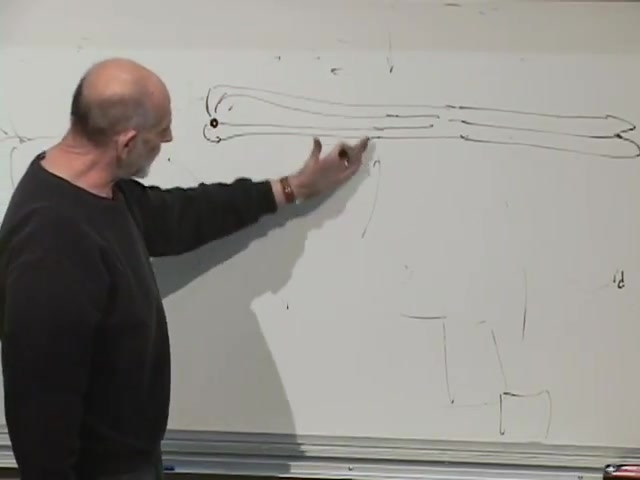
\includegraphics[width=0.78\textwidth]{lecture_04_figure_06.png}
\caption{クォークと反クォークの間に長い管として束ねられたカラーフラックス。}
\lectureframe{01:31:35}
\end{figure}

これは大きさが\(1/R\)として減少するクーロンポテンシャルよりも強い。
色源をさらに引き離しても力は無限に弱まるわけではない。
管が長くなり、エネルギーが加えられ続けるのである。無限体積中の孤立した色電荷は、
終わりなく伸びる管を必要とし、したがって無限のエネルギーを必要とする。これが、
有限エネルギーの漸近状態を持ち得るのはカラー一重項のみであるという主張の操作的
内容である。
\editorialnote{弦張力の記法と明示的な長距離ポテンシャルは、一様なフラックス管が単位長さあたり一様なエネルギーを運ぶという出典の記述を定量的にする。}

\subsection{弦の切断とジェット}

メソン内部の一つのクォークに硬い衝突が当たったとしよう。そのクォークは
離れ始めるが、フラックス管はその背後で伸びる。クォークは運動エネルギーを失い、
引き戻されるかもしれない。より多くの場合、蓄えられた場のエネルギーが十分に
大きくなると、真空は新しいクォーク--反クォーク対を生成する。新しい反クォークは
逃げていくクォークに付いたフラックスを終端させ、新しいクォークは
元の反クォークに付いたフラックスを終端させる。一つの伸びた
一重項が二つの短い一重項になる。
\begin{equation}
(q\bar q)_{\mathrm{stretched}}
\longrightarrow
(q\bar q)+(q\bar q).
\label{eq:l4-string-breaking}
\end{equation}

\begin{figure}[htbp]
\centering
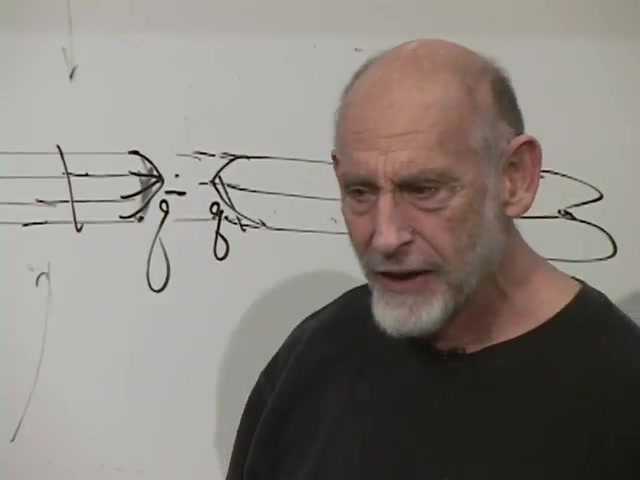
\includegraphics[width=0.78\textwidth]{lecture_04_figure_07.png}
\caption{対生成は一つの伸びたフラックス管を二つのカラー一重項の管に分ける。}
\lectureframe{01:34:52}
\end{figure}

\begin{classroomqa}
\audiencequestion{衝突されたクォークが管を伸ばし続けるのに十分なエネルギーを持つなら、引き戻される以外に何が起こり得るか。
\lecturetimestamp{01:33:50}}
\lecturerresponse{管はクォーク--反クォーク対生成によって切断され得る。そのエネルギーは新しい対の質量と運動エネルギーになる。端点は再結合して二つの一重項になるので、この過程は孤立したクォークではなく、追加のメソンを生成する。}
\end{classroomqa}

それらのパートンの一つが依然として大きな運動量を運ぶなら、過程は繰り返される。
結果は、元のパートンの方向の周りに集束したカラー一重項ハドロンのカスケード、すなわち
ジェットである。高エネルギーのクォークとグルーオンがハドロンに変換されるこの過程は
ハドロン化と呼ばれる。始まりとなった色を持つ対象は
ジェットから推論され、それ自体が観測されることは決してない。

\begin{classroomqa}
\audiencequestion{弦の切断はメソンだけを生成するのか、それとも他のハドロンもジェット中に現れ得るのか。
\lecturetimestamp{01:35:20}}
\lecturerresponse{他のハドロンも確かに現れ得る。唯一のカラーの要件は、最終的な観測可能な対象が一重項であることである。メソンは一回の切断に対する最も単純な描像であるが、バリオン、反バリオン、およびより複雑な一重項の組み合わせも生成され得る。}
\end{classroomqa}

三つのクォークはカラー一重項の接合部でそれらのフラックスを終端させ得る。この
三本の枝を持つ描像は、式~\eqref{eq:l4-baryon-singlet}の反対称
イプシロンテンソルの力学的対応物である。完全なバリオンから
正味のカラーフラックスは逃げない。

\begin{figure}[htbp]
\centering
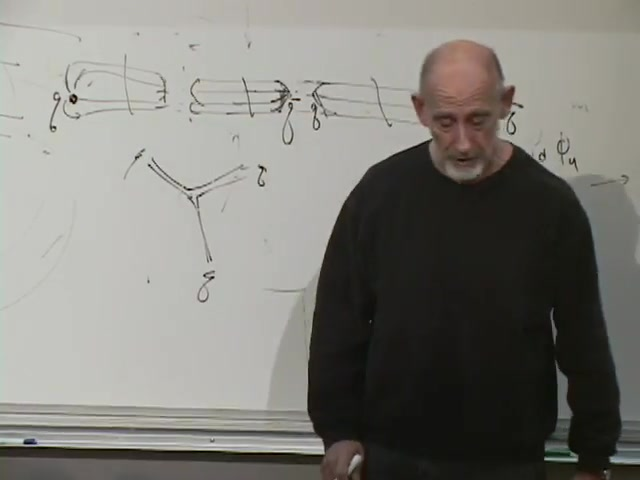
\includegraphics[width=0.72\textwidth]{lecture_04_figure_08.png}
\caption{バリオンのための三本の枝を持つカラーフラックス接合部。下はメソンの弦切断のスケッチ。}
\lectureframe{01:36:12}
\end{figure}

\section{ゲージ場、保存電荷、および標準模型}

現在の水準では、ゲージ理論は保存電荷が光子のような場の源となる理論として
認識され得る。電荷は電磁場の源であり、八つの色電荷は八つのグルーオン場の源である。
より深い定式化は対称性を局所化し、隣接する時空点における内部状態を比較する接続を
導入するが、その構成はここで展開した閉じ込めの描像には必要ない。
\editorialnote{局所対称性の定式化は、出典でほのめかされながら意図的に後回しにされたゲージ理論の標準的なより深い意味である。}

対称性、保存電荷、およびフラックスは密接に関係している。場の線が電荷でのみ
終わり得るなら、源が単に消え去り、そのフラックスが何にも付かないまま残ることはできない。
また、その遠方の場のすべてが瞬時に消えることもできない。場の変化は因果的に
伝播するからである。局所的な形では、同じ物理は連続の方程式
\begin{equation}
\frac{\partial\rho}{\partial t}
+\boldsymbol\nabla\cdot\boldsymbol j=0,
\end{equation}
によって表され、これは電荷がその境界を通って流れることによってのみ領域から
出て行き得ることを述べている。場の線による議論は、この局所保存則の幾何学的描像である。

これでこの結果を標準模型の中に位置づけることができる。カラーは\(SU(3)\)の8個の生成子とそれに対応する8個のグルーオン場を与える。アーベル部門は1個の生成子と1個のゲージ場を与える。さらに3個の生成子は、通常の空間角運動量ではなく、追加の\(SU(2)\)に属する。対称性の破れの前では、ゲージ構造は
\begin{equation}
SU(3)_c\times SU(2)_L\times U(1)_Y,
\end{equation}
であり、生成子の数は\(8+3+1=12\)個である。次の課題は、電弱\(SU(2)\)を理解し、次いでヒッグス場と、観測される光子、\(W^\pm\)、および\(Z\)がどのように現れるかを理解することである。
\editorialnote{原著者は光子を8個のグルーオンとともに数え、残りの因子を\(SU(2)\times U(1)\)と記述している。破れていない標準模型では、アーベル因子はハイパーチャージ\(U(1)_Y\)である。光子は電弱混合の後に初めて現れる。}

中心的な連鎖が今や完成した。抽象群は表現を通じて作用し、無限小生成子は保存電荷であり、クォーク、反クォーク、グルーオンはそれぞれ\(\boldsymbol 3\)、\(\bar{\boldsymbol 3}\)、\(\boldsymbol 8\)を占め、テンソル積が一重項ハドロンを同定し、非線形グルーオン場が一重項の選択を閉じ込めという物理現象へと変えるのである。